
\chapter{Machine Learning}

The term \textit{Machine Learning} was coined in 1959 by Arthur Samuel, an IBM employee and pioneer in the field of computer gaming and 
artificial intelligence.
The term \textit{Machine Learning} is often interchanged with other terms, such as \textit{Deep Learning}, \textit{Artificial Intellingence} (AI) 
and \textit{Artificial Neural Networks} (ANN), but they have different meanings.\\
The correct hierarchy among these terms is illustrated in Figure~\ref{fig:venn-AI}, where it is evident that the broadest term is AI and it includes 
\textit{Machine Learning}, \textit{Deep Learning}, and \textit{Artificial Neural Networks}.
A possible definition of AI was given by John McCarthy, an American computer scientist regarded as one of the founders of the field: 
\textit{"AI is the science and engineering of making intelligent machines."} (1956).

\begin{figure}[h]
\centering
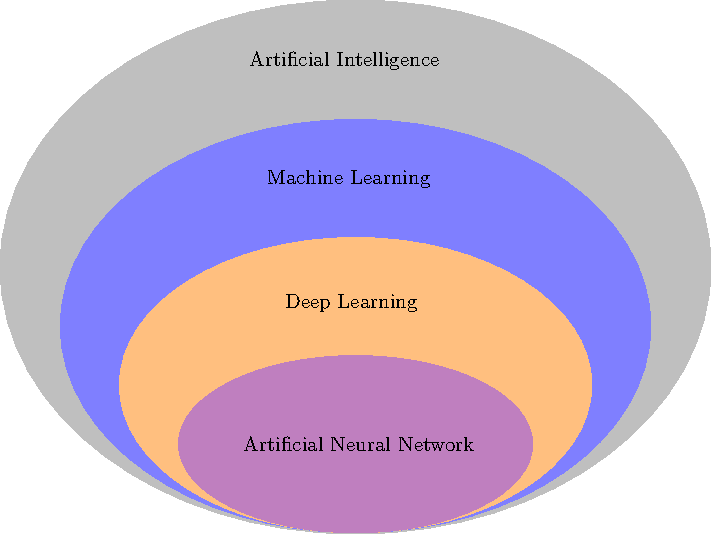
\includegraphics[scale=0.8]{sections/Chapters/Chapter2/venn_diagram/venn.pdf}
\caption{Venn diagram representing the relationship between AI, Machine Learning, Deep Learning and ANN.}
\label{fig:venn-AI}
\end{figure}

The distinction between \textit{Machine Learning} and \textit{Deep Learning} is often overlooked, but the key difference lies 
in the complexity and depth of the architectures. \textit{Deep Learning} models feature deep, layered architectures, while \textit{Machine Learning}
models typically involve shallower architectures. Today, nearly every model with significant real-world applications is a \textit{Deep Learning} model.\\

The term \textit{Machine Learning} refers to more than 60 different algorithms and they can be divided in three main categories: 

\begin{enumerate}

\item \textbf{Supervised Learning}: the algorithm learns to map an input to an output,  based on example input-output pairs.
Two main tasks belong to this category: classification and regression;
\item \textbf{Unsupervised Learning}: the algorithm learns patterns from untagged data.
Two main tasks belong to this category: clustering, dimensionality reduction;
\item \textbf{Reinforcement Learning}: the algorithm learns from the actions of an agent in an environment.
Its main task is real-time decisions;

\end{enumerate}

The operative workflow of a \textit{Machine Learning} model could be summarized by a \textit{pipeline} of five modules:

\begin{enumerate}

\item Data collection and cleaning;
\item Choice of the model, the cost function and the optimizer;
\item Training of the model;
\item Cross-Validation of the model;
\item Optimisation;

\end{enumerate}

\begin{figure}[h]
\centering
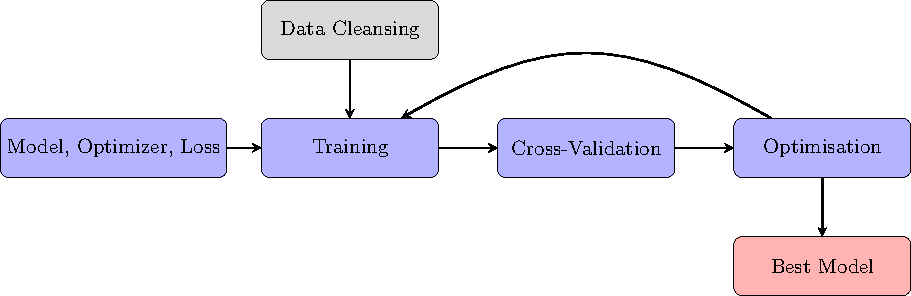
\includegraphics[scale=0.8]{sections/Chapters/Chapter2/flowchart.pdf}
\caption{Pipeline of a machine learning algorithm.}
\label{fig:pipeline}
\end{figure}

I will provide a detailed explanation of these five steps within the context of supervised learning, which has been the central focus of my thesis.

\section{Supervised Learning}

Supervised learning is one of the three main categories of machine learning algorithms.
Its task is to infer a function of certain variables in order to predict other variables.

As shown in figure~\ref{fig:pipeline} the \textit{pipeline} specific to a supervised learning algorithm has different steps.\\

The first step is the \textit{collection}, \textit{evaluation} and \textit{cleaning} of the data.\\
It is essential to study, understand, clean and assemble the training data.
The term \textit{data cleaning} or \textit{data cleansing} refers to all kinds of tasks and activities to detect and repair errors in the data.\\

The second step is the \textit{choice} of the model, the metric and the optimizer.\\
This choice depends on the specific task.
For instance, two possible model choices for a classification task are: Artificial Neural Networks or Boosted Decision Trees.\\
Many different metrics exist and it is essential to choose the most appropriate for the specific problem.\\
The most popular optimisation algorithms are \textit{gradient-descent} based (Adam, Nadam, ...).
The basic idea underlying these algorithms is to find a minimum (local or global) of the loss function through an iterative process.
Therefore, the first step is to select a starting point, an initial vector $\vec{\omega}_0$, and then the algorithm keeps updating the vector of 
parameters $\vec{\omega}$ (or weights of the model) until it finds a minimun of the loss function.\\
Gradient-based optimisation algorithms update iteratively the weights of the model with this simple rule:

\begin{equation}
\omega_{t} := \omega_{t-1} - \alpha \frac{\partial}{\partial \omega_{t-1}} J(\vec{\omega}_{t-1})
\label{eq:update-param}
\end{equation}

where $\alpha$ is the \textit{learning rate} and t indicates the iteration.
The \textit{learning rate} is a tuning parameter which determines the step size at each iteration while moving toward a minimum of the loss function.
It represent the \textit{learning speed} of a machine learning model.
It is essential to carefully choose the learning rate, since, if $\alpha$ is too small gradient descent could be really slow, if $\alpha$ is 
too large gradient descent may fail to converge or diverge. \\
Gradient-based optimization algorithms (such as Adam, Nadam, Adamax, ...) differ from one another by introducing slight variations to the parameter 
update equation~\ref{eq:update-param}.
Among these, the most widely used is Adam (Adaptive Moment Estimation) \cite{kingma2017}, which dynamically adjusts 
the learning rate for each parameter by estimating the first and second moments (mean and variance) 
of the gradients. The parameter update rule in Adam is given by:

\begin{equation}
    \omega_{t} := \omega_{t-1} - \alpha \frac{\hat{m}_t}{\sqrt{\hat{v}_t} + \epsilon} 
\end{equation}

where $\epsilon$ is a small constant added for numerical stability to prevent division by zero errors, whereas
The terms $\hat{m}_t$ and $\hat{v}_t$, as defined in the full Adam algorithm~\ref{work:adam}, represent bias-corrected estimates of the first 
and second moments of the gradients:

\begin{align}
    \hat{m}_t = \frac{m_t}{1 - \beta_1^t}
    \qquad
    \hat{v}_t = \frac{v_t}{1 - \beta_2^t}
\end{align}

$m_t$ and $v_t$ are the exponentially weighted moving averages of the gradients and the squared gradients, respectively.
The hyperparameters $\beta_1$ and $\beta_2$ control the decay rates of these moving averages, with $\beta_1^t$ and $\beta_2^t$ representing 
these values at the timestep $t$.\\

\begin{algorithm}
    \caption{Adam, an algorithm for stochastic optimization. $g_t^2$ indicates the elementwise
    square $g_t \odot g_t$. Good default settings for machine learning problems are $\alpha = 0.001$,
    $\beta_1 = 0.9$, $\beta_2 = 0.999$ and $\epsilon = 10^{-8}$. All operations on vectors are element-wise. With $\beta_1^t$ and $\beta_2^t$
    I denote $\beta_1$ and $\beta_2$ to the power t.}
    \label{alg:adam}
    \begin{algorithmic}
    \Require $\alpha$: Stepsize
    \Require $\beta_1$, $\beta_2$ $\in [0, 1)$: Exponential decay rates for the moment estimates
    \Require $f(\omega)$: Stochastic objective function with parameters $\omega$
    \Require $\omega_0$: Initial parameter vector
    \State $m_0 \gets 0$ (Initialize $1^{st}$ moment vector)
    \State $v_0 \gets 0$ (Initialize $2^{nd}$ moment vector)
    \State $t \gets 0$ (Initialize timestep)
    \While{$\theta_t$ not converged}
    \State $t \gets t + 1$
    \State $g_t \gets \nabla_{\omega} f_t(\omega_{t-1}) $ (Get gradients w.r.t. stochastic objective at timestep t)
    \State $m_t \gets \beta_1 \cdot m_{t-1} + (1 - \beta_1) \cdot g_t$ (Update biased first moment estimate)
    \State $v_t \gets \beta_2 \cdot v_{t-1} + (1 - \beta_2) \cdot g_t^2$ (Update biased second raw moment estimate)
    \State $\hat{m}_t \gets m_t / (1 - \beta^t_1)$ (Compute bias-corrected first moment estimate)
    \State $\hat{v}_t \gets v_t / (1 - \beta^t_2)$ (Compute bias-corrected second raw moment estimate)
    \State $\omega_t \gets \omega_{t-1} - \alpha \cdot \hat{m_t} / (\sqrt{\hat{v_t}} + \epsilon)$ (Update parameters)
    \EndWhile
    \State \Return $\theta_t$ (Resulting parameters)
\end{algorithmic}
\label{work:adam}
\end{algorithm}

The third step is the \textit{training} of the chosen model.\\
In this stage the model is provided with observed data (x) and the label of the data (y), also known as \textit{target values}.
By providing to the model observed data (x) and the label of the observed data (y), the algorithm learns and adapts to map observed data to the labeled data.
For instance, in the training stage of an animal classifier algorithm, x would be images of animals and y the animal breed, hence the algorithm 
learns to connect the right label to a specific animal.\\

The fourth step is \textit{Cross-Validation}.\\
The input dataset is typically divided into two primary subsets: the \textit{training} set and the \textit{testing} set. 
The model will have an associated error for each of these subsets: one for the training dataset and another for the testing dataset.
However, in most cases, the dataset is further divided into three subsets: the \textit{training} set, the \textit{validation} set, and 
the \textit{testing} set. The inclusion of the \textit{validation} set addresses the issue of the \textit{bias–variance trade-off}.
The \textit{bias–variance trade off} is the conflict in trying to simultaneously minimize the bias error and the variance error.
Supposing we have model $\hat{y}(x)$ determined from a training data set, and considering as the true model:

\begin{equation}
    Y = y(x) + \epsilon
\end{equation}

where the noise $\epsilon$ has zero mean and constant variance.
Given a test set sample ($x_0$,$y_0$), the expected squared error can be expressed as:

\begin{equation}
    E[(y_0 - \hat{y}(x_0))^2] = (Bias[\hat{y}(x_0)])^2 + Var[\hat{y}(x_0)] + Var(\epsilon) 
\label{eq:variance-bias}
\end{equation}

where:

\begin{align}
Bias[\hat{y}(x0)] = E[\hat{y}(x_0)] - y(x_0)
\qquad
Var[\hat{y}(x_0)] = E[\hat{y}(x_0)^2] - (E[\hat{y}(x_0)])^2
\label{eq:variance-bias-errors}
\end{align}

Here, $Bias[\hat{y}(x0)]$ represents the bias of the model's prediction $\hat{y}(x_0)$ relative to the true value $y_0$, while 
$Var[\hat{y}(x_0)]$ indicates the variance of the model's predictions. The term $Var(\epsilon)$ represents the variance of the noise in the data.\\
Our objective is to minimize the expected squared error as described in equation~\ref{eq:variance-bias}.\\
High bias typically results in \textit{underfitting}, where the model fails to capture important relationships between the 
features and the target outputs, leading to poor performance on both training and test data. On the other hand, high 
variance results in \textit{overfitting}, where the model learns the noise in the training data rather than 
the underlying patterns, which impairs its performance on new, unseen data.
Therefore, the goal is to strike an optimal balance between bias and variance to avoid both underfitting and overfitting. 
This involves selecting a model that captures the true underlying patterns in the data without being too sensitive to fluctuations 
in the training data.\\
In order to reduce the \textit{bias–variance trade off} it is common to use cross-validation techniques, 
which divide the dataset in three groups: \textit{training} set, \textit{validation} set and \textit{testing} set.

\begin{figure}[h]
\centering
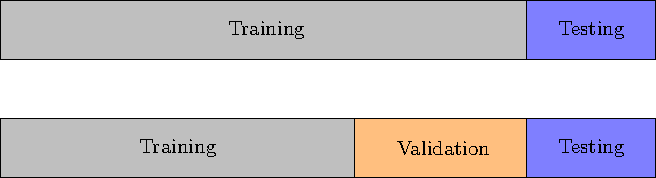
\includegraphics[scale=0.8]{sections/Chapters/Chapter2/cross.pdf}
\caption{Comparison between the division of the data in two sets and three sets.}
\end{figure}

An example of a cross-validation technique is \textit{k-fold}.\\
This technique consists in splitting the training dataset in N folds (groups), where N-1 sets are unified and become the new \textit{training} set 
and the last one becomes the \textit{validation} set.
In rotation every single k-fold will be used as the \textit{validation} set once.\\

\begin{figure}[h]
\centering
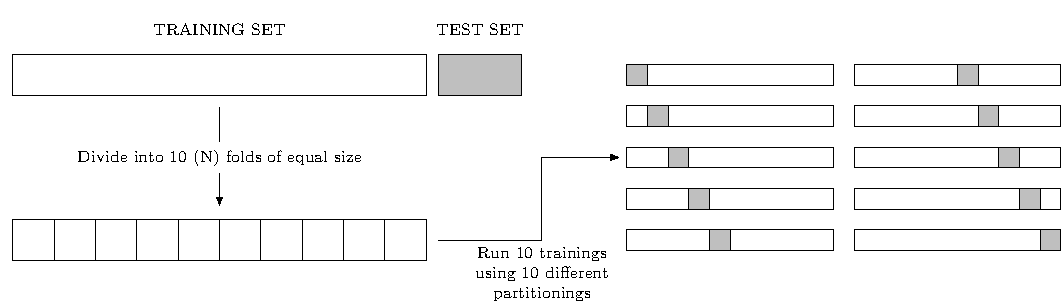
\includegraphics[scale=0.7]{sections/Chapters/Chapter2/kfold.pdf}
\caption{Schematic explanation of the k-fold cross validation technique with 10 folds.}
\end{figure}


Finally, the fifth and last step is \textit{Optimization}. This step involves exploring the space of \textit{hyperparameters} to find the best 
configuration for the model. It typically includes adjusting parameters such as learning rates, batch sizes, and regularization terms to improve 
model performance and ensure optimal results.\\
Some common techniques for hyperparameter optimization are:

\begin{enumerate}
    \item Grid Search.\\
    Grid search involves defining a set of possible values for each hyperparameter and then exhaustively searching through all 
    possible combinations of these values.
    The great advantage of this technique is that it is easy to implement.
    However it can be unfeasible, because exploring every possible combination could be too computationally expensive.

    \item Random Search.\\
    Random search involves sampling hyperparameter values randomly from predefined distributions. Unlike grid search, 
    it does not evaluate all possible combinations but rather selects a subset of random configurations.
    It is often more efficient than grid search because it can explore a larger and more diverse set of combinations with fewer evaluations.
    The main disadvantage is that there is no guarantee that the best configuration will be found, as it only samples a subset of the 
    possible combinations.

    \item Genetic Algorithms.\\
    Genetic algorithms (for further informations \cite{alam2020}) are inspired by the process of natural selection. They evolve a population of hyperparameter configurations 
    over multiple generations, using operations like mutation, crossover, and selection to find the best configurations.
    The main disadvantages are that it can be computationally expensive and it requires the tuning of internal parameters.

    \item Bayesian optimization.\\
    Bayesian optimization (for further informations \cite{frazier2018}) uses a probabilistic model to predict the performance of different hyperparameter configurations. 
    It iteratively selects the most promising configurations to evaluate based on past results, aiming to find the optimal set more efficiently.
    It can be more efficient than Grid Search and Random Search, but it requires a careful choice of the probabilistic model.

\end{enumerate}

In conclusion, the third, fourth and fifth steps can be repeated until the \textit{Best Model} is found.


\section{Artificial Neural Networks}

\textit{Artificial neural networks} (ANNs) are computing systems inspired by the biological neural networks that constitute animal brains.\\
An ANN can be visualised as \textit{layers} of \textit{neurons} (or \textit{node}), each of which receives inputs from all neurons in the previous layer.
A neural network has an \textit{input} and an \textit{output} layer and the layers in between are referred to as \textit{hidden}.
When the number of hidden layers (the network \textit{depth}) goes beyond one, the network is normally referred to as \textit{deep neural network} (DNN). 
The number of neurons in a given layer is referred to as its \textit{width}.

\begin{figure}[h]
\centering
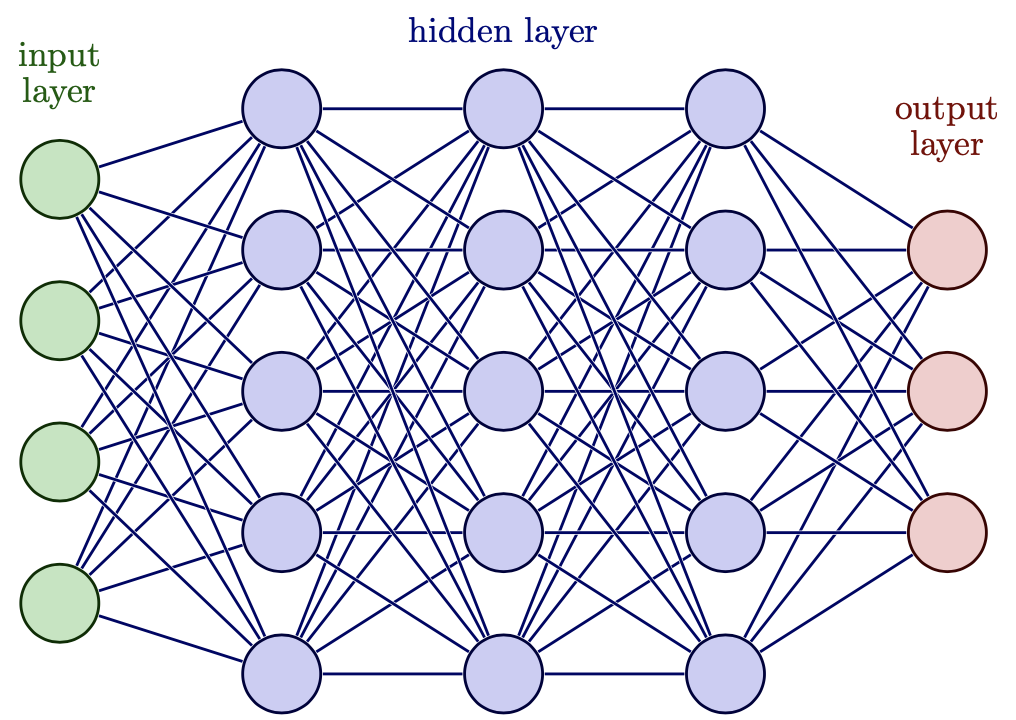
\includegraphics[scale=0.5]{sections/Chapters/Chapter2/foto.png}
\caption{Multilayer perceptron with three hidden layers.}
\end{figure}

The neuron (or perceptron) is the fundamental unit of every ANN.
Each node combines linearly the input with \textit{weights} and a \textit{bias} and then its output is modulated by an \textit{activation function}, which introduces the non-linearity in the model.
Therefore the output of a node would be:

\begin{equation}
a = g(w_{0} + w_{1} x_1 + w_{2} x_2 + w_{3} x_3)
\end{equation}

where g is the activation function, $w_{0}$ is the bias and $w_{i}$ ($i \ne 0$) are the weights.

\begin{figure}[h]
\centering
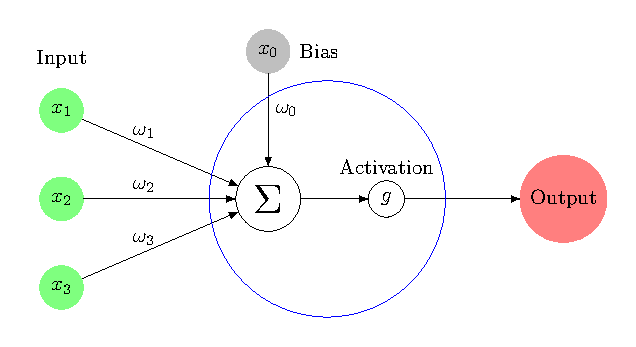
\includegraphics[scale=1]{sections/Chapters/Chapter2/neuron.pdf}
\caption{Schematic representation of a neuron.}
\end{figure}


Many different activation functions exist: \textit{tanh}, \textit{sigmoid}, \textit{ReLU}, \textit{ELU}, ...\\
The training of an ANN is usually performed with gradient descent methods.
Since the number of weights could be copious, it is essential to use an algorithm which reduces the large amount of computations.
The \textit{backpropagation algorithm} is the most common algorithm to compute the gradient, since it can be used with any gradient-based optimizer.\\

There is a wide range of artificial neural network (ANN) architectures, ranging from simple models like the single perceptron to more complex ones 
such as Generative Adversarial Networks (GANs). Figure~\ref{fig:zoo} provides a partial overview of the diverse spectrum of neural network architectures.

\subsection{Multilayer Perceptron}

A Multilayer Perceptron (MLP) is the builiding block of many ANN architectures.\\
It is a \textit{fully-connected} and \textit{feed-forward} artificial neural network.
The term \textit{fully-connected} means that each node of a layer is connected with every node of the previous layer.
The term \textit{feed-forward} means that connections between nodes do not form a cycle or a loop, hence the information moves in only 
one direction (forward) from the input nodes, through the hidden nodes and to the output nodes.


\subsection{Convolutional Neural Network}

Convolutional Neural Networks (CNNs) are a class of deep neural networks specifically designed to process and analyze grid-like data structures, 
such as images. CNNs are the standard architecture for tasks such as image 
classification, object detection, and image generation.\\

A CNN has two main components:

\begin{itemize}
    \item Convolutional Layer.\\
    Convolutional layers perform a convolution operation using filters (or kernels).
    Each kernel is a matrix of learnable weights that are updated during training.
    Each filter slides over the image with a certain stride (step size). At each position, 
    an element-wise multiplication (equation~\ref{eq:filter}) is performed between the filter and the portion of the input data it covers:

    \begin{equation}
        (I * K)(i,j)= \sum_m \sum_n I(i+m,j+n) \cdot K(m,n)
    \label{eq:filter}
    \end{equation}

    where (i,j) represents the position in the output feature map, and (m,n) indexes the filter matrix.
    This process enables the network to detect spatial hierarchies and essential features from the data.

    \begin{figure}[h]
    \centering
    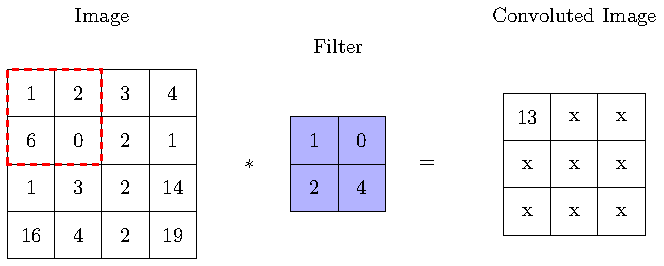
\includegraphics[scale=0.7]{sections/Chapters/Chapter2/convolution/convolution.pdf}
    \caption{Convolution operation.}
    \end{figure}

    \item Pooling Layer.\\
    Pooling layers reduce the spatial dimensions of the feature maps while preserving important information. Common pooling techniques, 
    like max pooling and average pooling, help in minimizing computational complexity and making the network less sensitive to small translations 
    and distortions in the input data.

    \begin{figure}[h]
    \centering
    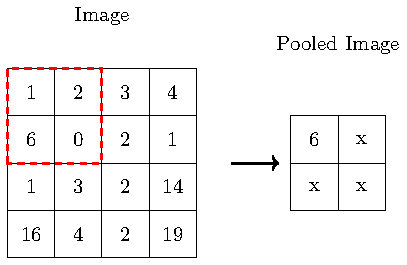
\includegraphics[scale=0.7]{sections/Chapters/Chapter2/pooling/pooling.pdf}
    \caption{Max pooling operation.}
    \end{figure}
\end{itemize}

Following several convolutional and pooling layers, the high-level features are flattened and passed through a multilayer perceptron, which is
responsible for making final predictions based on the learned features.


\subsection{Binary and Multi-Class Classification}

Classification problems are supervised learning tasks for predicting variables that consist of a finite number of categories called
\textit{classes}. 
When the number of classes is two the classification problem is called \textit{binary-classification}, when the number of classes is larger than
two, the classification problems are called \textit{multi-class classification} problems. \\
Many different models could be used to deal with a classification task, such as K-Nearest Neighbors, Decision
Trees or Artificial Neural Networks.\\
The next two paragraphs describe the main features of binary and multi-class classifiers using as model an ANN.



\subsection{Binary Classifier}

A binary classifier distinguishes between two classes and therefore has a single node in the output layer. The output of this 
node is a probability score ranging from 0 (indicating the first class) to 1 (indicating the second class). To make a final 
classification decision, a \textit{discrimination threshold} must be set. This threshold determines the point at which the probability score is 
converted into a binary classification, effectively deciding which class the input belongs to based on the predicted probability.
A possible choice for the cost function of a binary classifier is the \textit{binary cross-entropy}:

\begin{equation}
J(\vec{\omega}) = - \frac{1}{n} \sum_{i=1}^n y_i log(\hat{y}_\omega(x_i)) + (1-y_i)(log(1-\hat{y}_\omega(x_i)))
\end{equation}

where $y_i$ is the target value, $\hat{y}_\omega(x_i)$ is the model output:

\begin{equation}
\hat{y}_{\omega}(x_i) = \frac{1}{1+e^{-\omega^Tx_i}}
\end{equation}

The output of a binary classifier can be visualized in a \textit{confusion matrix}.

\begin{figure}[h]
\centering
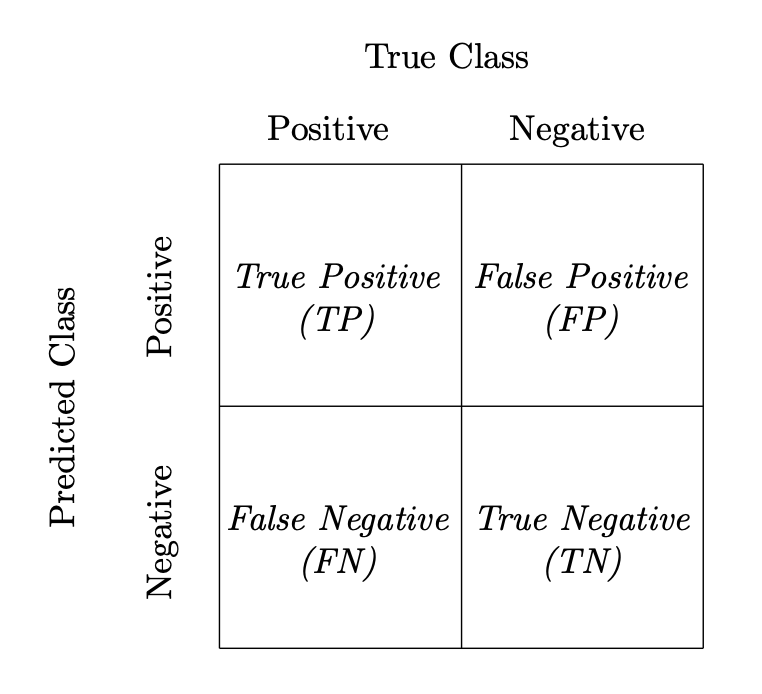
\includegraphics[scale=0.5]{sections/Chapters/Chapter2/confusionmatrixdef.png}
\caption{Confusion matrix for a binary classifier.}
\end{figure}

Each row of the \textit{confusion matrix} represents the instances in a \textit{predicted class} while each column represents the instances 
in a \textit{true class} (or vicecersa).
In binary classification tasks the cost function is usually complemented with many other metrics based on the \textit{confusion matrix}:

\begin{itemize}

\item Accuracy:

\begin{equation}
Accuracy = \frac{TP + TN}{TP + TN + FP + FN}
\end{equation}

\item Precision:

\begin{equation}
Precision = \frac{TP}{TP + FP}
\end{equation}

\item Recall (or True positive rate):

\begin{equation}
Recall = \frac{TP}{TP + FN}
\end{equation}

\item False positive rate:

\begin{equation}
Recall = \frac{FP}{FP + TN}
\end{equation}

\item F1 score:

\begin{equation}
F1 = 2 \cdot \frac{Precision \cdot Recall}{Precision +  Recall}
\end{equation}

\end{itemize}

However these metrics depend on the discrimination threshold.
Therefore it is useful to introduce metrics which show the diagnostic ability of a binary classifier system as its discrimination threshold is varied:

\begin{itemize}

\item The \textit{ROC curve} plots the true positive rate against the false positive rate at various threshold settings;
\item The \textit{AUC} is the integral of the ROC curve;

\end{itemize}


\subsection{Multi-class Classifier}
\label{section:multiclass_explanation}

There are two main strategies for solving a multi-class classification problem. 
The first is the use of classification algorithm which can solve the problem directly (K-Nearest Neighbors, Decision
Trees, Artificial Neural Networks). 
The second strategy is the decomposition of the original multi-class classification problem 
into several binary sub-problems (one-against-one or one-against-rest), and each sub-problem can be solved with a different 
classification algorithm.\\

A multi-class classifier has one node per class in the output layer.\\
Unlike a binary classifier whose output is modulated by a sigmoid, a multi-class network has as output a \textit{softmax} output. 
The \textit{softmax} function takes as input the vector of values of the output layer and converts them into probabilities associated to each class. 
Therefore the output of \textit{softmax} is a probability vector of three components for a multi-class classifier with three classes.

\begin{equation}
\sigma_i(\vec{x}) = \frac{exp(x_i)}{\sum^N_{i=1} exp(x_j)}
\end{equation}

The sum of the components of the \textit{softmax} output vector is normalized to one by definition.\\
The cost function of a multi-class classifier is the \textit{categorical cross-entropy}:

\begin{equation}
J(\vec{\omega}) = - \sum_{i=1}^{n} y_i log(\hat{y}_{\omega}(x_i))
\end{equation}


where $y_i$ is the i-th element of the vector $\vec{y}$ (the target vector) and represents the actual class, meanwhile $\hat{y}_{\omega}(x_i)$ represents the value of the i-th output.
The target vectors $\vec{y}$ for a three class classifier are three, one for each class:



\begin{align}
\vec{y}_1 = \begin{pmatrix}
1\\
0\\
0
\end{pmatrix}
\qquad
\vec{y}_2 = \begin{pmatrix}
0\\
1\\
0
\end{pmatrix}
\qquad
\vec{y}_3 =\begin{pmatrix}
0\\
0\\
1
\end{pmatrix}
\end{align}





